\documentclass{book}

% Configuration
% ------------------
% Packages
% ------------------
\usepackage[english]{babel}
\usepackage[T1]{fontenc}
\usepackage[scaled]{helvet}
\usepackage[utf8]{inputenc}
\usepackage[letterpaper, margin=1in]{geometry}
\usepackage[dvipsnames]{xcolor}

\usepackage{algorithm}
\usepackage{algorithmicx}
\usepackage{algpseudocode}
\usepackage{amsfonts,amsmath,amsthm,amssymb}
\usepackage{booktabs}
\usepackage{float}
\usepackage{graphicx}
\usepackage{latexsym}
\usepackage{mathtools}
\usepackage{sectsty}
\usepackage{setspace}
\usepackage{subcaption}
\usepackage{tabularx}
\usepackage{tikz}
% \usepackage{txfonts}
\usepackage{url}
\usepackage{wrapfig}
\usepackage{xparse}

% ------------------
% Shortcuts
% ------------------
\newcommand{\R}{\mathbb{R}}
\newcommand{\N}{\mathbb{N}}

\newcommand{\id}{\mathrm{id}}

\newcommand{\Frontier}{\texttt{Frontier}}

% ------------------
% Command Redefinitions
% ------------------
\renewcommand{\qed}{\hfill$\blacksquare$}

\makeatletter
\renewcommand*\env@matrix[1][*\c@MaxMatrixCols c]{%
    \hskip -\arraycolsep
    \let\@ifnextchar\new@ifnextchar
    \array{#1}}
\makeatother

% ------------------
% Colors
% ------------------
\definecolor{primary}{HTML}{207BA5}
\definecolor{greybg}{RGB}{249, 249, 249}

\definecolor{thmbg}{HTML}{F2F2F9}
\definecolor{lemmabg}{HTML}{FFFAF8}
\definecolor{lemmafr}{HTML}{983b0f}
\definecolor{propbg}{HTML}{f2fbfc}
\definecolor{propfr}{HTML}{191971}
\definecolor{myp}{RGB}{197, 92, 212}
\definecolor{grey17}{RGB}{17, 17, 17}
\definecolor{MyGrey}{HTML}{5B5B5B}

\definecolor{lightBlue}{rgb}{0.0, 0.64, 1.0}
\definecolor{lightRed}{rgb}{1.0, 0.50, 0.50}
\definecolor{darkGreen}{rgb}{0.31, 0.54, 0.30}
\definecolor{violet}{RGB}{186, 153, 242}

%----------------
%	Text Styles
%----------------
\DeclareTextFontCommand{\term}{\color{orange}\bfseries}
\DeclareTextFontCommand{\bred}{\color{red}\bfseries}
\DeclareTextFontCommand{\itblue}{\color{lightBlue}\itshape}

\DeclareTextFontCommand{\vector}{\bfseries\itshape}

% ------------------
%   URL Color
% ------------------
\usepackage[colorlinks=true]{hyperref}
\hypersetup{
    colorlinks=true,
    linkcolor=black,
    filecolor=magenta,
    urlcolor=blue,
}

% ------------------
% Tikz Externalize
% ------------------
\usetikzlibrary{external}
\tikzexternalize[prefix=tikz/]
\tikzset{external/only named=true}

% ------------------
% Boxes
% ------------------
\usepackage[most]{tcolorbox}

\newcommand\fancybox[3]{%
    \tcbset{
        mybox/.style={
                enhanced,
                boxsep=0mm,
                opacityfill=0,
                overlay={
                        \coordinate (X) at ([xshift=-1mm, yshift=-1.5mm]frame.north west);
                        \node[align=right, text=#1, text width=2.5cm, anchor=north east] at (X) {\bf#2};
                        \draw[line width=0.5mm, color=#1] (frame.north west) -- (frame.south west);
                    }
            }
    }
    \begin{tcolorbox}[mybox]
        #3
    \end{tcolorbox}
}

\tcbuselibrary{theorems,skins,hooks}
\NewDocumentCommand\thmbox{m O{\Large #1} O{greybg} O{primary} O{number within=section}}
{
    \newtcbtheorem[#5]{#1}{\large #2}
    {%
        enhanced,
        breakable,
        colback = #3,
        frame hidden,
        boxrule = 0sp,
        borderline west = {2pt}{0pt}{#4},
        sharp corners,
        detach title,
        before upper = \tcbtitle\par\smallskip,
        coltitle = #4,
        fonttitle = \bfseries,
        %description font = \mdseries,
        separator sign none,
        segmentation style={solid, #4}
    }
    {th}
}

\thmbox{Corollary}[Corollary][myp!10][myp!85!black]
\thmbox{Lemma}[Lemma][lemmabg][lemmafr]
\thmbox{Propo}[Proposition][propbg][propfr]
\thmbox{Defi}[Definition][primary!12][primary]
\thmbox{Notation}[Notation][white][grey17][no counter]
\thmbox{Theorem}[Theorem][primary!12][primary]
\thmbox{Remark}[Remark][grey17!10][grey17][no counter]

% ------------------
% Environments
% ------------------
\newenvironment{corollary}[1][]   {\begin{Corollary}{#1}{}}                               {\end{Corollary}}
\newenvironment{definition}[1][]  {\begin{Defi}{#1}{}}                                    {\end{Defi}}
\newenvironment{lemma}[1][]       {\begin{Lemma}{#1}{}}                                   {\end{Lemma}}
\newenvironment{proposition}[1][] {\begin{Propo}{#1}{}}                                   {\end{Propo}}
\newenvironment{remark}[1][]      {\begin{Remark}{#1}{}}                                  {\end{Remark}}
\newenvironment{theorem}[1][]     {\begin{Theorem}{#1}{}}                                 {\end{Theorem}}

\newenvironment{rtheorem}[2][]    {\begin{Theorem}{#1}{#2}}                               {\end{Theorem}}

\theoremstyle{definition}
\newtheorem*{exam}{\color{primary}Example}
% \newcommand{\example}[1]{\begin{exam}#1\end{exam}}
% \newenvironment{example}          {\begin{exam}} {\begin{flushright}${\color{primary}\diamondsuit}$\end{flushright} \end{exam}}
\newenvironment{example}          {\begin{exam}} {\hfill${\color{primary}\diamondsuit}$\end{exam}}

\theoremstyle{definition}
\newtheorem*{clm}{\color{MyGrey}Claim}
\newenvironment{claim}            {\begin{clm}} {\end{clm}}

% ------------------
% Lists
% ------------------
\usepackage{enumitem}

\newcommand{\cnumero}[2]{
    \tikz[baseline=(myanchor.base)]
    \node[minimum size=0.2cm,circle,
        inner sep=1pt,draw, #2,thick,fill=#2](myanchor)
    {\color{white}\bfseries\fontsize{8}{8}#1};}

\newcommand*{\itembolasazules}[1]{\protect\cnumero{#1}{primary}}

\newenvironment{listo} {\begin{enumerate}[label=\itembolasazules{\arabic*}]} {\end{enumerate}}
\newenvironment{listu} {\begin{itemize}  [label=$\color{primary} \bullet$]}  {\end{itemize}}

% ------------------
% Table of Contents
% ------------------
\usepackage{blindtext}
\usepackage{framed}
\usepackage{titletoc}
\usepackage{etoolbox}

\patchcmd{\tableofcontents}{\contentsname}{\contentsname}{}{}

\renewenvironment{leftbar}
{\def\FrameCommand{\hspace{6em}%
        {\color{primary}\vrule width 2pt depth 6pt}\hspace{1em}}%
    \MakeFramed{\parshape 1 0cm \dimexpr\textwidth-6em\relax\FrameRestore}\vskip2pt%
}
{\endMakeFramed}

\titlecontents{chapter}[0em]
{\vspace*{2\baselineskip}}
{\parbox{4.5em}{%
        \hfill\Huge\bfseries\color{primary}\thecontentslabel}%
    \vspace*{-2.3\baselineskip}\leftbar\textbf{\color{primary}\small\chaptername~\thecontentslabel}\\
}{}{\endleftbar}

\titlecontents{section}[8.4em]
{\contentslabel{3em}}{}{}
{\hspace{0.5em}\nobreak\itshape\color{primary}\contentspage}

\titlecontents{subsection}[11.4em]
{\contentslabel{3em}}{}{}
{\hspace{0.5em}\nobreak\itshape\color{primary}\contentspage}

% ------------------
% Chapters
% ------------------
\newtcolorbox{titlecolorbox}[1]{ %the box around chapter
    coltext=white,
    colframe=primary,
    colback=primary,
    boxrule=0pt,
    arc=0pt,
    notitle,
    width=4.8em,
    height=2.4ex,
    before=\hfill
}

\usepackage[explicit]{titlesec}

\makeatletter
\let\old@rule\@rule
\def\@rule[#1]#2#3{\textcolor{primary}{\old@rule[#1]{#2}{#3}}}
\makeatother

\titleformat{\chapter}[display]
{\Huge}
{}
{0pt}
{\begin{titlecolorbox}{}
        {\large\MakeUppercase{\bf\chaptername}}
    \end{titlecolorbox}
    \vspace*{-3.19ex}\noindent\rule{\textwidth}{0.4pt}
    \parbox[b]{\dimexpr\textwidth-4.8em\relax}{\raggedright\MakeUppercase{#1}}{\hfill\fontsize{70}{60}\selectfont{\color{primary}\thechapter}}
}
[]

\titleformat{name=\chapter,numberless}[display]
{\Huge}
{}
{0pt}
{
    \vspace*{-3.19ex}\noindent\rule{\textwidth}{0.4pt}
    \parbox[b]{\dimexpr\textwidth-4.8em\relax}{\raggedright\MakeUppercase{#1}}
}
[]

% ------------------
% Sections
% ------------------
\titleformat{\section}[hang]{\Large\bfseries}%
{\rlap{\color{primary}\rule[-6pt]{\textwidth}{0.4pt}}\colorbox{primary}{%
        \raisebox{0pt}[13pt][3pt]{ \makebox[60pt]{% height, width
                \selectfont\color{white}{\thesection}}
        }}}%
{15pt}%
{ \color{primary}#1
    %
}
\titlespacing*{\section}{0pt}{3mm}{5mm}
% ------------------
% Subsections
% ------------------
\subsectionfont{\Large\color{primary}}

% ------------------
% Bibliography and Index
% ------------------
\usepackage{csquotes}
\usepackage[
    style=alphabetic, 
    citestyle=numeric,
    sorting=nyt,
    sortcites=true,
    autopunct=true,
    autolang=hyphen,
    hyperref=true,
    abbreviate=false,
    backref=true,
    backend=biber,
    defernumbers=true
]{biblatex}
\addbibresource{./bibliography.bib} % BibTeX bibliography file
\defbibheading{bibempty}{}

\usepackage{calc} % For simpler calculation - used for spacing the index letter headings correctly
\usepackage{makeidx} % Required to make an index
\makeindex % Tells LaTeX to create the files required for indexing

% ------------------
% Title page
% ------------------
\usetikzlibrary{calc}
\usetikzlibrary{shapes.geometric}
\usepackage{anyfontsize}
\newcommand{\frontpage}[3]{
    \begin{tikzpicture}[remember picture, overlay]
        % Background
        \fill[primary] (current page.south west) rectangle (current page.north east);

        \foreach \i in {2.5,...,22} {
            \node[rounded corners,primary!60,draw,regular polygon,regular polygon sides=6, minimum size=\i cm,ultra thick] at ($(current page.west)+(2.5,-5)$) {} ;
        }

        % Background Polygon
        \foreach \i in {0.5,...,22} {
            \node[rounded corners,primary!60,draw,regular polygon,regular polygon sides=6, minimum size=\i cm,ultra thick] at ($(current page.north west)+(2.5,0)$) {} ;
        }

        \foreach \i in {0.5,...,22} {
            \node[rounded corners,primary!90,draw,regular polygon,regular polygon sides=6, minimum size=\i cm,ultra thick] at ($(current page.north east)+(0,-9.5)$) {} ;
        }

        \foreach \i in {21,...,6} {
            \node[primary!85,rounded corners,draw,regular polygon,regular polygon sides=6, minimum size=\i cm,ultra thick] at ($(current page.south east)+(-0.2,-0.45)$) {} ;
        }

        % Title
        \node[left,primary!5,minimum width=0.625*\paperwidth,minimum height=3cm, rounded corners] at ($(current page.north east)+(0,-9.5)$) {
            {\fontsize{25}{30} \selectfont \bfseries #1}
        };

        % Subtitle
        \node[left,primary!10,minimum width=0.625*\paperwidth,minimum height=2cm, rounded corners] at ($(current page.north east)+(0,-11)$) {
            {\huge \textit{#2}}
        };

        % Author
        \node[left,primary!5,minimum width=0.625*\paperwidth,minimum height=2cm, rounded corners] at ($(current page.north east)+(0,-13)$) {
            {\Large \textsc{#3}}
        };

        % Year
        \node[rounded corners,fill=primary!70,text =primary!5,regular polygon,regular polygon sides=6, minimum size=2.5 cm,inner sep=0,ultra thick] at ($(current page.west)+(2.5,-5)$) {\LARGE \bfseries \the\year{}};
    \end{tikzpicture}
}


\begin{document}

\pagestyle{empty}
\frontpage{CSC384}{Introduction to Artificial Intelligence}{Sinan Li}
\newpage

\tableofcontents
\newpage

\tikzset{
    graph-node/.style={
        circle,
        fill=red,
        draw=black,
        line width=0.5pt,
        inner sep=1.5pt
    },
    every edge/.style={
        draw,
        thick,
    },
    non-edge/.style={
        dotted,
        lightBlue,
    },
}

\part{Notes}

\chapter{Introduction to Artificial Intelligence}

\section{Artificial Intelligence (AI)}

Artificial Intelligence is a branch of computer science utilizing \itblue{computational} ideas and examining how we can achieve \itblue{intelligent} behavior through computation. 

\subsection{Intelligence}

\textit{The ability to apply knowledge to manipulate one's environment or to think abstractly as measured by objective criteria (such as tests)}
\begin{flushright}
    \textit{--- Merriam-Webster Dictionary}
\end{flushright}

Human features that are considered intelligent includes the ability to learn, understand, reason, plan, communicate, and perceive. For example, a human can learn to play a game, understand the rules of the game, reason about the best moves to make, plan a sequence of moves, communicate with other players, and perceive the state of the game.

\subsection{The Turing Test}

The Turing Test is a test of a machine's ability to exhibit intelligent behavior equivalent to, or indistinguishable from, that of a human. The test was introduced by Alan Turing in his 1950 paper, \textit{Computing Machinery and Intelligence}, while working at the University of Manchester \cite{10.1093/mind/LIX.236.433}. Turing proposed that a human evaluator would judge natural language conversations between a human and a machine designed to generate human-like responses. The evaluator would be aware that one of the two partners in conversation is a machine, and all participants would be separated from one another. The conversation would be limited to a text-only channel such as a computer keyboard and screen so that the result would not be dependent on the machine's ability to render words as speech. If the evaluator cannot reliably tell the machine from the human, the machine is said to have passed the test. The test does not check the ability to give the correct answer to questions; it checks how closely the answer resembles typical human answers. The conversation is limited to a single topic chosen by the examiner. 

\begin{listu}
    \item Turing provided some very persuasive arguments that a system passing the Turing test is \itblue{intelligent}.

    \begin{listu}
        \item We can only really say it \itblue{behaves} like a human
        \item \bred{No guarantee} that it \itblue{thinks} like a human
    \end{listu}

    \item The Turing test does not provide much traction on the question of \bred{how to build} an intelligent system.
\end{listu}

\subsubsection{Why not just simulate human's brain?}

\begin{listu}
    \item Brains are very good at making rational decisions, but \bred{not perfect}.
    \item Brains \bred{aren't as modular} as software, so hard to reverse engineer!
    \item Computers and Humans have quite \bred{different abilities}.
    \begin{listu}
        \item \itblue{Memory} and \itblue{simulation} are key to decision making.
        \item \itblue{Perceptual tasks} (vision, sound, etc.) are effectively accomplished by architectures related to the way the brain works (deep neural networks).
    \end{listu}
\end{listu}

\subsection{Computational Intelligence}

Artificial Intelligence tries to understand and model \itblue{intelligence} as a \bred{computational process}. Thus we try to construct systems whose \bred{computation} achieves or approximates the desired notion of intelligence.

Other areas interested in the study of intelligence lie in other areas or study, e.g., cognitive science which focuses on human intelligence. Such areas are very related, but their central focus tends to be different.

\section{Rationality}

Formally, we can define an \term{agent} as something that \bred{perceives} and \bred{acts} in an \itblue{environment}. An agent can be a \itblue{human}, a \itblue{robot}, or a \itblue{software agent}.

A \term{rational agent} is one that acts so as to achieve the best outcome or, when there is uncertainty, the best expected outcome. Rationality is distinct from omniscience (knowing everything) and omnipotence (being able to do anything). Rationality maximizes \term{expected utility}, which is the sum of the utility of each possible outcome of an action weighted by its probability of occurring. 

Rationality is measured by the \itblue{outcome}, not the \itblue{action} itself. It is a precise \itblue{mathematical} notion of of what it means to do \itblue{the right thing} in any particular circumstance. Provides
\begin{listu}
    \item A \bred{precise mechanism} for analyzing and understanding the properties of this ideal behaviour we are trying to achieve.
    \item A \bred{precise benchmark} against which we can measure the behaviour the systems we build.
\end{listu}

\subsubsection{Trying/Expectation}

Rational action is not always equal to rational decision. 

\begin{listo}
    \item We often don't have \bred{full control} or \bred{knowledge} of the world we are interacting with.
    \item We usually don't know \bred{precisely} what the \bred{effects} of our actions will be.
\end{listo}

In some contexts we can \itblue{simplify} the computational task by assuming that we do have full knowledge/control.

\section{Subareas of AI}

A common misconception is to equate AI with Machine Learning. But AI is much more than that. This course will not focus on Machine Learning, but rather on the other subareas of AI. What we cover is not an exhaustive list of all subareas of AI, but rather a starting point for further exploration.

\begin{listu}
    \item \textbf{Perception}: vision, speech understanding, etc.
    \item \textbf{Machine Learning}, \textbf{Neural Networks}
    \item \textbf{Robotics}
    \item \textbf{Natural Language Processing}
    \item \textbf{Reasoning and Decision Making}
    \begin{listu}
        \item \textbf{Symbolic Knowledge Representation}
        \item \textbf{Reasoning} (logical, probabilistic)
        \item \textbf{Decision Making} (search, planning, decision theory)
    \end{listu}
\end{listu}

\subsection{Further Courses in AI}

\begin{listu}
    \item Perception: vision, speech understanding, etc.
    \begin{listu}
        \item CSC487H1 ``Computational Vision''
        \item CSC420H1 ``Introduction to Image Understanding''
    \end{listu}

    \item Machine Learning, Neural networks
    \begin{listu}
        \item CSC311H ``Introduction to Machine Learning''
        \item CSC412H ``Probabilistic Learning and Reasoning''
        \item CSC413H1 ``Neural Networks and Deep Learning''
    \end{listu}

    \item Robotics
    \begin{listu}
        \item Engineering courses
    \end{listu}

    \item Natural language processing
    \begin{listu}
        \item CSC401H1 ``Natural Language Computing''
        \item CSC485H1 ``Computational Linguistics''
    \end{listu}

    \item Reasoning and decision making
    \begin{listu}
        \item CSC486H1 ``Knowledge Representation and Reasoning''
    \end{listu}
\end{listu}

\section{A Brief History of AI}

\begin{listu}
    \item 1940-1950: Early days
    \begin{listu}
        \item 1943: McCulloch \& Pitts: Boolean circuit model of brain
        \item 1950: Turing's “Computing Machinery and Intelligence”
    \end{listu}

    \item 1950—70: Excitement: Look, Ma, no hands!
    \begin{listu}
        \item 1950s: Early AI programs, including Samuel's checkers program, Newell \& Simon's Logic Theorist, Gelernter's Geometry Engine
        \item 1956: Dartmouth meeting: “Artificial Intelligence” adopted
        \item 1965: Robinson's complete algorithm for logical reasoning
    \end{listu}

    \item 1970—Early 2000: Knowledge-based approaches
    \begin{listu}
        \item 1969—79: Early development of knowledge-based systems
        \item 1980—88: Expert systems industry booms
        \item 1988—93: Expert systems industry busts: “AI Winter”
        \item 1997: IBM's Deep Blue beats chess grandmaster Garry Kasparov
    \end{listu}

    \item Early 2000— present: Statistical approaches
    \begin{listu}
        \item Resurgence of probability, focus on uncertainty
        \item Agents and learning systems… “AI Spring”
        \item 2007: DARPA Urban Challenge -- CMU autonomous vehicle drives 55 miles in an urban environment while adhering to traffic hazards and traffic laws.
        \item 2016: AlphaGo beats 9-Dan pro Go player Lee Sedol
        \item 2017: AlphaGo Zero -- learns by playing with itself
        \item 2022: Large Language Models (LLM) Chat Generative Pre-trained Transformer, which has been fueled by advances in Neural Net architecture and access to big data. 
    \end{listu}
\end{listu}

There are many \bred{unsolved} problems yet\dots including lots of \bred{legal/ethical} ones. 
\chapter{Search}

\section{Search Problems}

Searching is one of the most \itblue{fundemental techniques} in AI, underlying sub-module in many AI systems. Ai can \itblue{solve} many problems that homansare not good at, and achieve \itblue{super-human performance} in many domains (e.g. chess, go, etc.).

\begin{listu}
    \item \textbf{Benefits}

    \begin{listu}
        \item Useful as ageneral algorithmic technique for solving problems, both in AI and in other areas.

        \item Outperform humans in some areas (e.g. games). 

        \item Practical:

        \begin{listu}
            \item Many problems don't have specific algorithms for solving them.
            \item Useful in approximation (e.g., local search in optimization problems).
        \end{listu}

        \item Some critical aspects of intelligent behaviour, e.g., planning, can be cast as search.
    \end{listu}
    
    \item \textbf{Limitations}
    
    \begin{listu}
        \item Only shows how to solve the problem once we have it correctly formulated.
    \end{listu}
\end{listu}

% TODO: Planning and Scheduling Problems:

\subsection{Formalizing a Problem as a Search Problem}

\begin{listu}
    \item Necessary components
    
    \begin{listo}
        \item \bred{State Space}: A \term{state} is a representation of a \itblue{configuration} of the problem domain. The state space is the \itblue{set of all states} include in our model of the problem. 
        \item \bred{Initial State}: The starting configuration. 
        \item \bred{Goal State}: The configuration one wants to achieve. 
        \item \bred{Actions} (or State Space Transitions): Allowed changed to move from one state to another. 
    \end{listo}

    \item Optional Ingredients 
    
    \begin{listu}
        \item \itblue{Costs}: Representing the cost of moving from state to state. 
        \item \itblue{Heuristics}: Help guide the search process. 
    \end{listu}
\end{listu}

Once a search problem is formalized, there are a number of algorithms one can use to solve it. A \term{solution} is a \itblue{sequence of actions} or moves that can transform the \bred{initial state} into a \bred{goal state}. 

\begin{example}[Romania Travel]
    We want to travel in Romania from Arad to Bucharest as fast as possible. 

    \begin{center}
        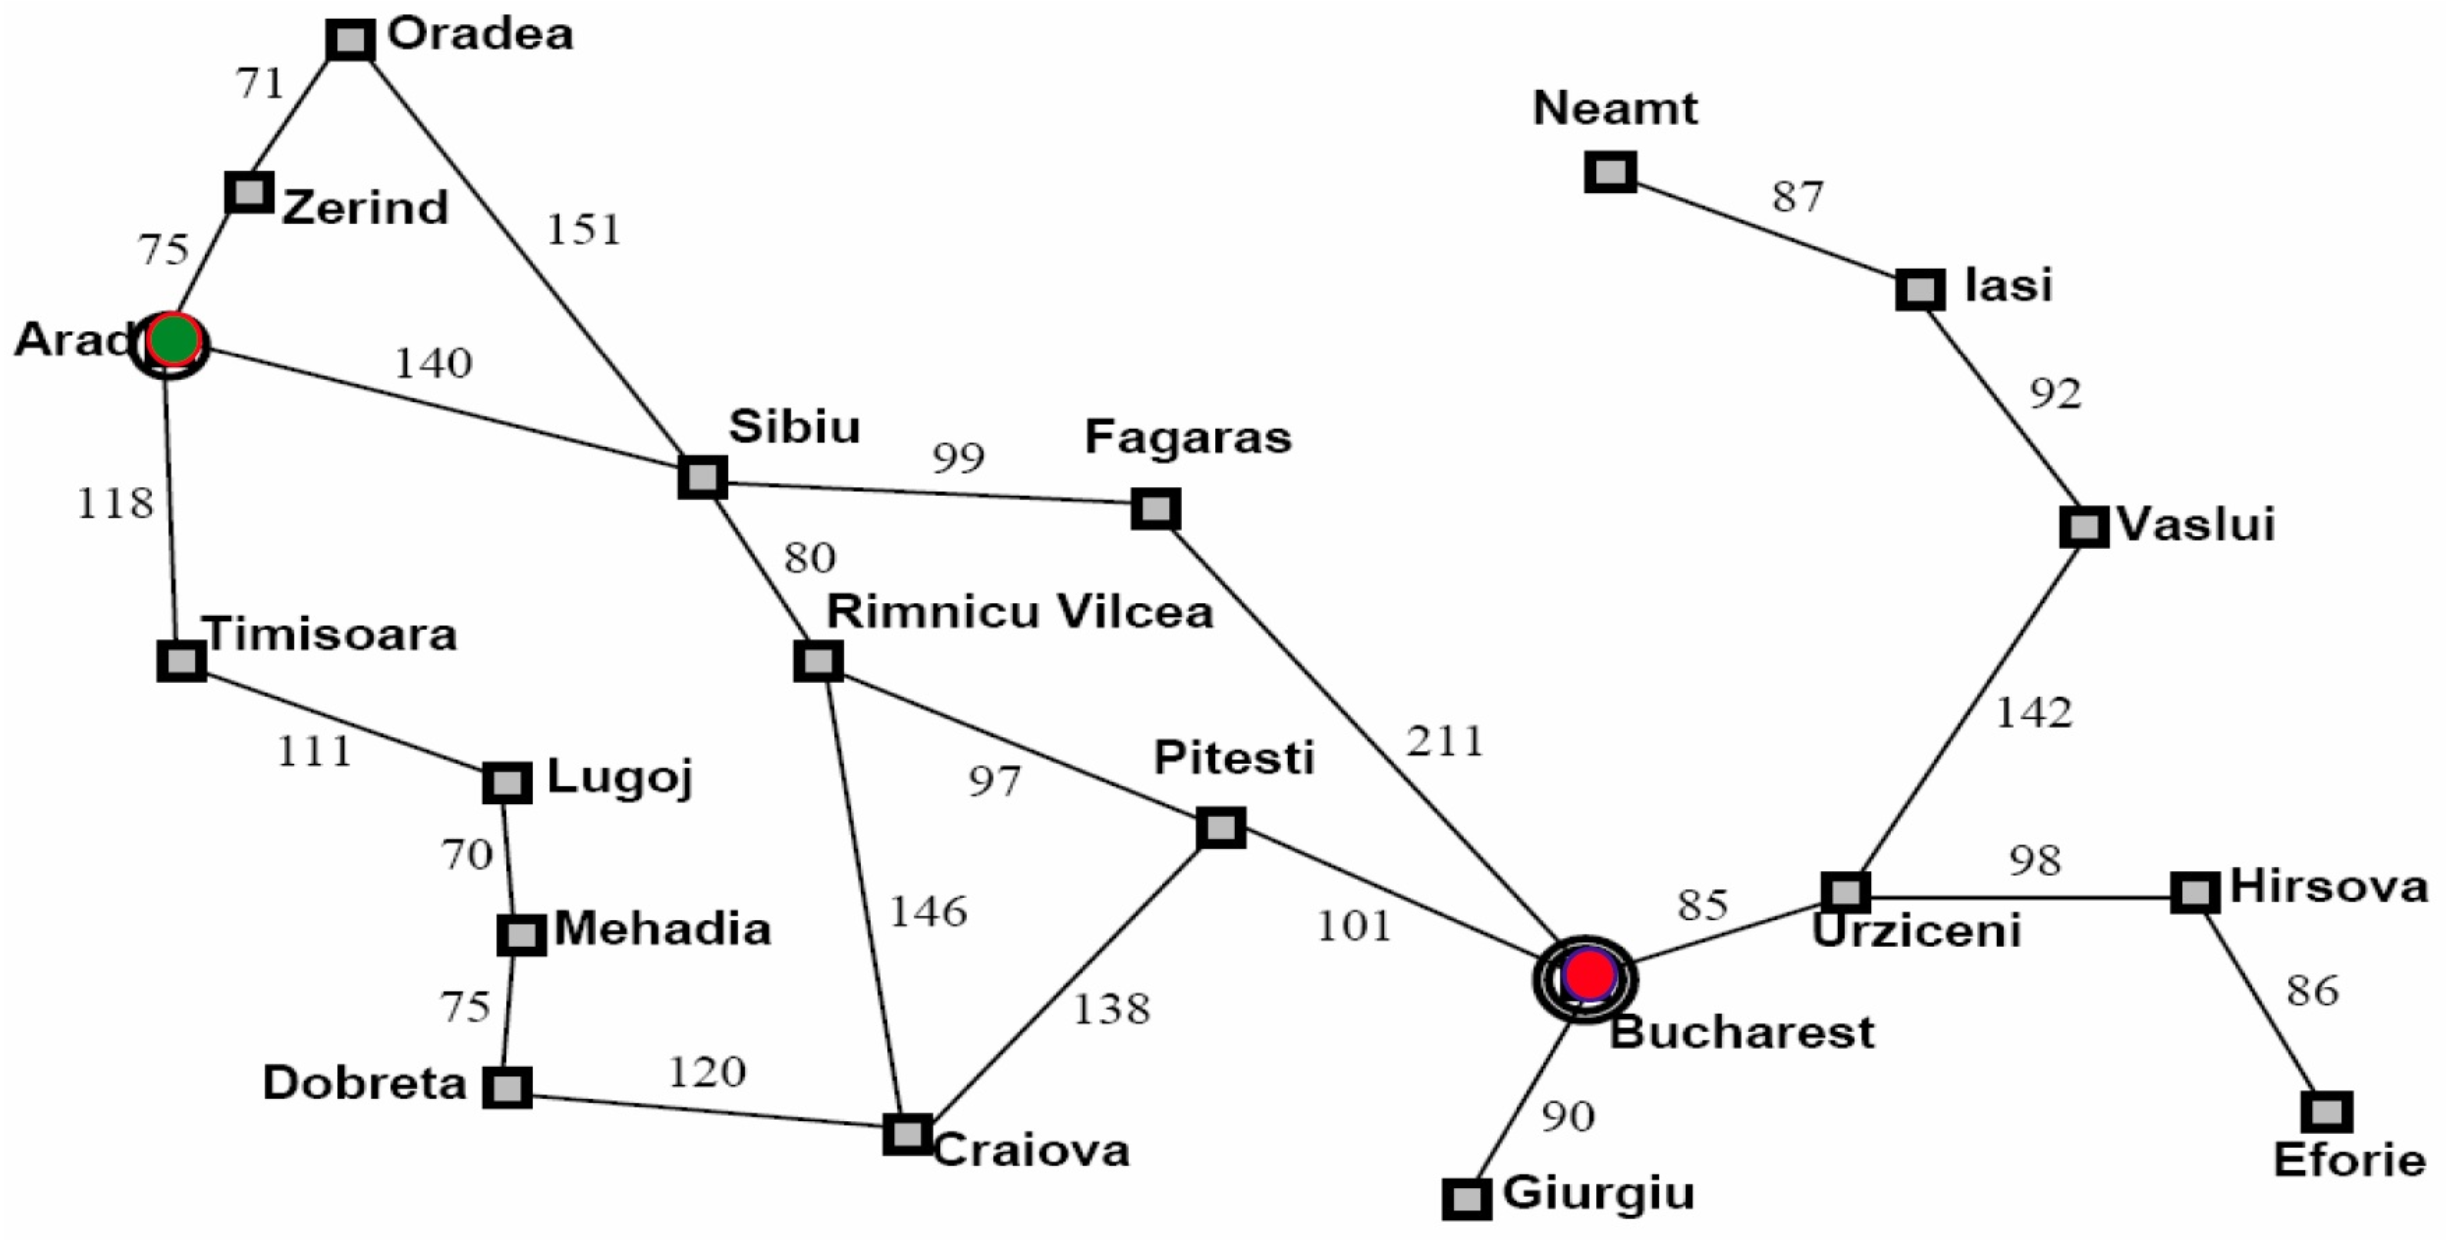
\includegraphics[width=0.75\linewidth]{figures/Romania Travel.png}
    \end{center}

    Each state would be a city. 

    \begin{listu}
        \item \bred{State Space}: The set of all cities on the map.
        \item \bred{Initial State}: Arad.
        \item \bred{Goal State}: Bucharest.
        \item \bred{Actions}: Driving between neighbouring cities.
    \end{listu}
\end{example}

\begin{example}[Water Jugs]
    We have a 3-liter jug and a 4-liter jug. We can fill either jug to the top from a tap, or we can empty either jug onto the ground. We can also pour the contents of one jug into the other until the receiving jug is full or the pouring jug is empty.

    Suppose initially the 4-liter jug is full, we want to have exactly 2 liters in the 3-liter jug.

    {~~~}

    We can use a pair of numbers to represent the state of the system: the amount of water in the 3-liter jug and the amount of water in the 4-liter jug.

    \begin{listu}
        \item \bred{State Space}: The set of all pairs of numbers $(a, b)$ where $a$ is the amount of water in the 3-liter jug and $b$ is the amount of water in the 4-liter jug.
        \item \bred{Initial State}: $(0, 4)$.
        \item \bred{Goal State}: $(2, 0)$, $(2, 1)$, $(2, 2)$, $(2, 3)$, $(2, 4)$.
        \item \bred{Actions}: 
        \begin{listu}
            \item Fill the 3-liter jug from the tap.
            \item Fill the 4-liter jug from the tap.
            \item Empty the 3-liter jug onto the ground.
            \item Empty the 4-liter jug onto the ground.
            \item Pour the contents of the 3-liter jug into the 4-liter jug.
            \item Pour the contents of the 4-liter jug into the 3-liter jug.
        \end{listu}
    \end{listu}

    \begin{remark}
        When formalizing a search problem, always consider these questions:

        \begin{listo}
            \item Can we reach all states fron any given start state?

            \item Will all actions result in a change of state? 

            \bred{No!} Imagine you have $(3, 4)$ and you try to fill the 3-liter jug from the tap. You will still have $(3, 4)$.
        \end{listo}
    \end{remark}
\end{example}

\subsubsection{More Complex Situations}

In more complex situations, 

\begin{listu}
    \item Actions may lead to \bred{multiple states}. 
    
    For example, filpping a coin may lead to heads or tails.

    \item We may not be \bred{sure of a given state}
    
    For example, when prize is behind door 1, 2, or 3.

    \item Such situations require techniques for reasoning under uncertainty: assign probabilities to given outcomes.
\end{listu}

\subsection{Graphical Representation}

\begin{center}
    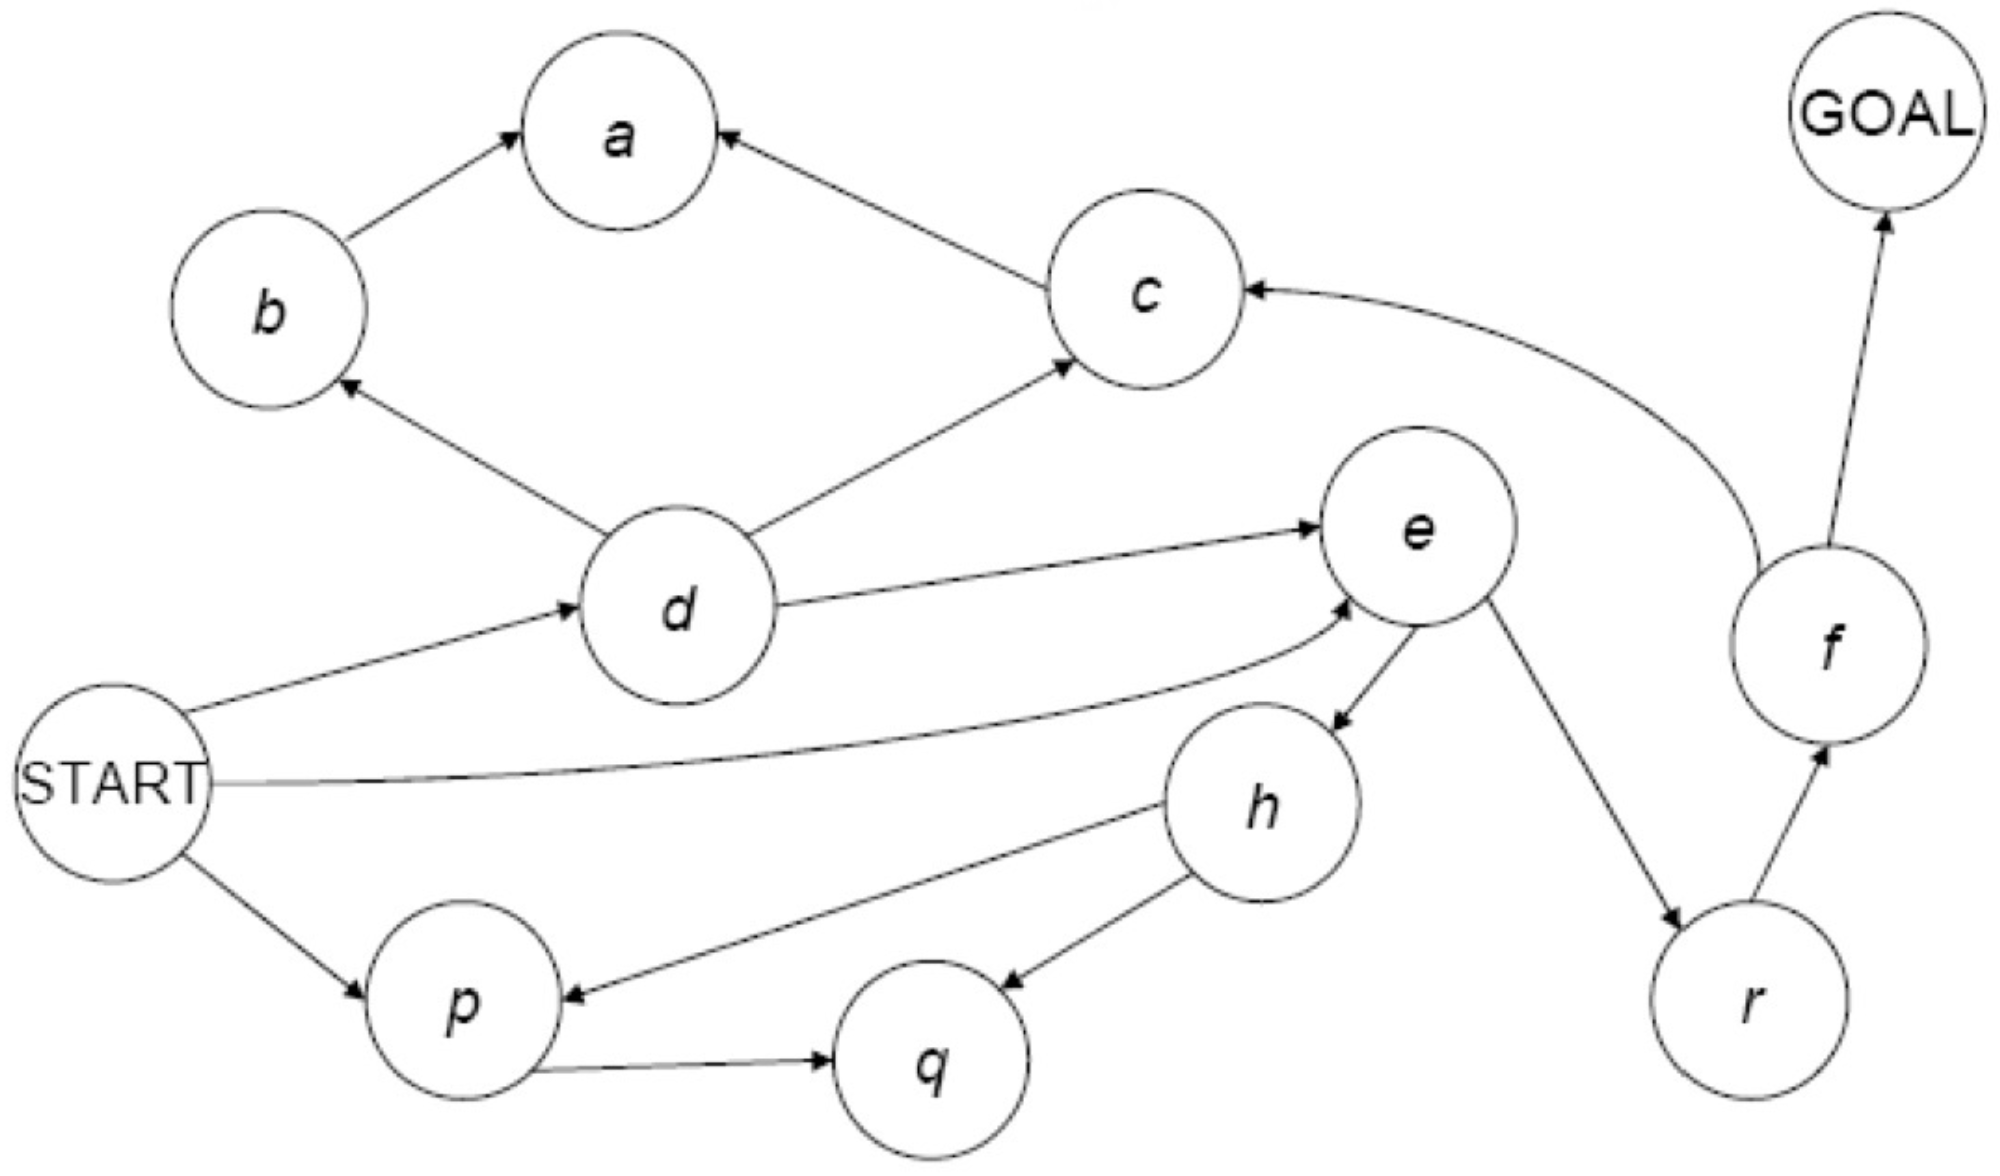
\includegraphics[width=0.67\linewidth]{figures/Search Graph Rep.png}
\end{center}

Assuming a finite search space, the

\begin{listu}
    \item \bred{vertices} represent states in the search space; and the 
    \item \bred{edges} represent transitions resulting from actions (or successor functions).
\end{listu}

\subsubsection{Search Tree}

\begin{definition}[Search Tree]
    A \term{search tree} is a \itblue{directed graph} where

    \begin{listu}
        \item Each node represents a state.
        \item Each edge represents an action.
        \item The root node represents the initial state.
        \item The leaf nodes represent goal states.
    \end{listu} 
\end{definition}

A search tree reflects the behaviour of an algorithm as it walks through a search problem. It has two important properties:

\begin{listu}
    \item \term{Solution depth}, denoted $d$, the depth of the shallowest goal node in the tree.
    \item \term{Maximum branching factor}, denoted $b$, the maximum number of children of any node in the tree.
\end{listu}

\begin{remark}
    Note that the \bred{same} state may appear \bred{multiple times} in a search tree.
\end{remark}

\begin{remark}
    It is important to distinguish between \bred{states} from \bred{nodes}. 

    \begin{listu}
        \item A \bred{state} represents a possible configuration of the world. 
        \item A \itblue{node} is a data structure constituting part of a search tree. It includes 
        \begin{listu}
            \item a \bred{state} and 
            \item the \bred{parent node}, 
            \item the \bred{action} that led to this node, and 
            \item the \bred{cost} of the path from the initial node to this node. 
        \end{listu}
        \item  Intuitively speaking, each node corresponds with a path from the initial state to the node's state.
        \item Two \bred{different nodes} are allowed to contain the \bred{same world state}.
    \end{listu}
\end{remark}

\subsection{Algorithms for Search}

\begin{listu}
    \item \textbf{Input}
    
    \begin{listu}
        \item \textbf{Initial node}

        \item \textbf{Successor Function} $S(x)$
        
        returns the set of nodes that can be reached from node $c$ via a single action. 

        \item \textbf{Goal Test Function} $G(x)$
        
        returns true if node $c$ satisfies the goal condition. 

        \item \textbf{Action Cost Function} $C(x, a, y)$
        
        returns the cost of moving from node $x$ to node $y$ using action $a$.

        Note that $C(x, a, y) = \infty$ if $y$ is not reachable from $a$ via $a$. 
    \end{listu}

    \item \textbf{Output}
    
    \begin{listu}
        \item A \itblue{sequence of actions} that transforms the initial node satisfying the goal test. 
        \item The sequence might be, \term{optimal in cost} for some algorithms, \term{optimal in length} for some algorithms, come with \bred{no optimality} guarantees from other algorithms.
    \end{listu}

    \item \textbf{Procedure}
    
    \begin{listu}
        \item Put nodes have not yet expanded in a list called the \term{\texttt{Frontier}} (or \term{Open}).
        \item Initially, only the \itblue{initial node} is in the \texttt{Frontier}.
        \item At each iteration, pull a node from the \texttt{Frontier}, apply $S(x)$, and insert the children back into the \texttt{Frontier}.
        \item Repeat until pulling a goal node.
    \end{listu}
\end{listu}

\newpage
\begin{algorithm}
    \caption{Tree Search Algorithm}
    
    \begin{algorithmic}[1]
        \Function{TreeSearch}{Frontier, Successors, Goal?}
            % If frontier is empty, return failure
            \If{Frontier is empty}
                \State \Return failure
            \EndIf

            \State Curr $\gets$ select state from frontier

            \If{Goal?(Curr)}
                \State \Return Curr
            \EndIf

            \State Frontier' $\gets$ Frontier $-$ \{ Curr \} $\cup$ Successors(Curr)

            \State \Return \Call{TreeSearch}{Frontier', Successors, Goal?}
        \EndFunction
    \end{algorithmic}
\end{algorithm}

% TODO: example

Note that the search terminates only when a goal node is expanded into the \texttt{Frontier}.
\chapter{Game Tree Search}
\chapter{Constraint Satisfaction Problems}
\chapter{Representing and Reasoning under Uncertainty}
\chapter{Symbolic Knowledge Representation and Reasoning}

\part{Appendices}

\chapter*{Bibliography}
\addcontentsline{toc}{part}{Bibliography}
\nocite{*}
\printbibliography[heading=bibempty]

\cleardoublepage
\phantomsection
\setlength{\columnsep}{0.75cm}
\addcontentsline{toc}{part}{Index}
\printindex

\end{document}